\documentclass[ignorenonframetext,professionalfonts, hyperref={pdftex, unicode}]{beamer}

\usetheme{Copenhagen}
\usecolortheme{wolverine}

\usepackage[orientation=landscape, size=custom, width=16, height=9.75, scale=0.5]{beamerposter}	

%Packages to be included

\usepackage{textcomp}

\usepackage[russian]{babel}
\usepackage[utf8]{inputenc}
\usepackage[T1]{fontenc}

\usepackage{beamerthemesplit}

\usepackage{ulem}

\usepackage{verbatim}

\usepackage{ucs}
\usepackage{listings}
\lstloadlanguages{C, make, bash}

\lstset{escapechar=`,
	extendedchars=false,
	language=C, 
	tabsize=2, 
	columns=fullflexible, 
%	basicstyle=\scriptsize,
	keywordstyle=\color{blue}, 
	commentstyle=\itshape\color{brown},
%	identifierstyle=\ttfamily, 
	stringstyle=\mdseries\color{green}, 
	showstringspaces=false, 
	numbers=left, 
	numberstyle=\tiny, 
	breaklines=true, 
	inputencoding=utf8x,
	keepspaces=true,
	morekeywords={u\_short, u\_char, u\_long, in\_addr}
	}

\definecolor{darkgreen}{cmyk}{0.7, 0, 1, 0.5}

\lstdefinelanguage{diff}
{
    morekeywords={+, -},
    sensitive=false,
    morecomment=[l]{//},
    morecomment=[s]{/*}{*/},
    morecomment=[l][\color{darkgreen}]{+},
    morecomment=[l][\color{red}]{-},
    morestring=[b]",
}



%%%%%%%%%%%%%%%%%%%%%%%%%%%%%%%%%%%%%%%%%%%%%%%%%
%%%%%%%%%% PDF meta data inserted here %%%%%%%%%%
%%%%%%%%%%%%%%%%%%%%%%%%%%%%%%%%%%%%%%%%%%%%%%%%%
\hypersetup{
	pdftitle={Введение в GNU/Linux},
	pdfauthor={Epam/LLPD}
}





%%%%%% Beamer Theme %%%%%%%%%%%%%

	
\title{Введение в GNU/Linux}
\author{Epam/LLPD}



%%%%%%%%%%%%%%%%%%%%%%%%%%%%%%%%%%%%%%%%%%%%%%%%%
%%%%%%%%%% Begin Document  %%%%%%%%%%%%%%%%%%%%%%
%%%%%%%%%%%%%%%%%%%%%%%%%%%%%%%%%%%%%%%%%%%%%%%%%




\begin{document}

\section{Введение}


\frame{
	\frametitle{}
	\titlepage
	\vspace{-0.5cm}
	\begin{center}
	%\frontpagelogo
	\end{center}
}
\frame{
	\tableofcontents
%	[hideallsubsections]
}






%%%%%%%%%%%%%%%%%%%%%%%%%%%%%%%%%%%%%%%%%   
%%%%%%%%%% Content starts here %%%%%%%%%%
%%%%%%%%%%%%%%%%%%%%%%%%%%%%%%%%%%%%%%%%%

\mode<all>{\begin{frame}{Цель курса}
	\begin{center}
		\Huge
		Увеличение популярности GNU/Linux среди программистов.

		\hrulefill

		\normalsize
		Воспитание потенциальных сотрудников ;-)
	\end{center}
\end{frame}


\begin{frame}{Состав курса}
	\begin{itemize}
		\item Представление об архитектуре GNU/Linux дистрибутива
			\pause
		\item "Ежедневные" навыки работы в консоли
			\pause
		\item Введение в shell-программирование
			\pause
		\item Работа с классическими средствами разработки
			\pause
		\item Все, чего вы не знали и боялись спросить
	\end{itemize}
\end{frame}
}

\subsection{GNU/Linux}

\mode<all>{\begin{frame}{Терминология}
	\begin{itemize}
		\item GNU -- GNU's Not Unix!
		\begin{itemize}
			\item 1983. Ричард Столлман. Свободное ПО.
		\end{itemize}

		\pause

		\item POSIX
		\begin{itemize}
			\item 1988. Portable Operating System Interface for Unix. 
		\end{itemize}

		\pause

		\item Linux
		\begin{itemize}
			\item 1991. Линус Торвальдс. Ядро.
		\end{itemize}

	\end{itemize}
\end{frame}
}

\subsection{Лицензии}

\mode<all>{\begin{frame}{Лицензии: открытые и свободные}

	\begin{block}{ Р.Столлман: 4 свободы}

		\begin{itemize}
			\item Свобода 0: Свобода запускать программу в любых целях.
			\item Свобода 1: Свобода изучения работы программы и адаптация её к вашим нуждам. 
				Доступ к исходным текстам является необходимым условием.
			\item Свобода 2: Свобода распространять копии,  так что вы можете помочь вашему товарищу.
			\item Свобода 3: Свобода улучшать программу и публиковать ваши улучшения,
				так что всё общество выиграет от этого.
				Доступ к исходным текстам является необходимым условием.
		\end{itemize}
	\end{block}


\end{frame}

\begin{frame}{Copyleft }

	\begin{block}{ \textcopyleft  -- ``Копилефт''}
	Авторское лево -- концепция и практика использования законов авторского права для обеспечения 
	невозможности ограничить любому человеку право использовать,  изменять и распространять как 
	исходное произведение,  так и произведения,  производные от него.
	\end{block}


	При копилефте все производные произведения должны распространяться под той же лицензией,
	что и оригинальное произведение.

\end{frame}


\begin{frame}{Лицензии}
	\begin{itemize}
		\item GPL
		\item LGPL
		\item AGPL
		\item BSD
		\item MIT
		\item Mozilla Public License
		\item Apache Software License
		\item Creative Commons *
	\end{itemize}
\end{frame}
}

\section{Дистрибутивы ОС Linux}

\mode<all>{\begin{frame}{Дистрибутив ОС GNU/Linux}
	\begin{block}{ Определение}
		\pause
		Набор программного обеспечения на базе ядра Linux, распространяющийся как единое целое.
	\end{block}
\end{frame}


\begin{frame}{Задачи дистрибутива}
	\begin{itemize}
		\item Предоставление комплекта ПО (ядро + утилиты)
		\item Средства установки и настройки
		\item Средства обновления
	\end{itemize}
\end{frame}

\begin{frame}{Различия между дистрибутивами}

	\Large\center{\bf{Цели!!!}}

	\bigskip
	\normalsize

	\pause

	\begin{itemize}
		\begin{columns}
		\column{0.4\textwidth}
			\item Инсталлятор
			\item Первичные настройки
			\item Средства управления
			\item Набор ПО
		\column{0.4\textwidth}
			\item Менеджер пакетов
			\item Формат распространения ПО
			\item Пути к файлам
			\item Система сборки ПО
		\end{columns}
	\end{itemize}
\end{frame}

\begin{frame}{Дистрибутивы}
	\begin{itemize}
		\begin{columns}
		\column{0.3\textwidth}
			\item RedHat
			\item Fedora Core
			\item CentOS
			\item Scientific Linux
			\item Oracle Unbreakable Linux
		\column{0.3\textwidth}
			\item Slackware 
			\item Gentoo
			\item Arch
			\item OpenSUSE
			\item ALT Linux 
		\column{0.3\textwidth}
			\item Debian
			\item Ubuntu
			\item Mint
			\item Knoppix
			\item BackTrack
		\end{columns}
	\end{itemize}
\end{frame}
}

\section{Процесс загрузки ОС Linux}

\mode<all>{\begin{frame}{Процесс загрузки GNU/Linux}

	\begin{enumerate}
		\item BIOS
		\item MBR
			\pause
		\item Загрузка загрузчика
		\begin{itemize}
			\item Stage 1 -- Первичный загрузчик
			\item Stage 1,5 -- Загрузка ядра загрузчика и драйвера ФС
			\item Stage 2 -- Чтение конфигурации
		\end{itemize}
			\pause

		\item Загрузка ядра в память
		\item Загрузка initrd в память
			\pause
		\item Передача управления ядру
		\begin{itemize}
			\item Распаковка
			\item Инициализация
		\end{itemize}

		\item Монтирование initrd
		\item Запуск программы инициализации в initrd
			\pause
		\item Нахождение и монтирование корневого раздела
			\pause
		\item Запуск программы init
		\begin{itemize}
			\item Монтирование оставшихся разделов ФС
			\item Инициализация оборудования
			\item Запуск демонов
		\end{itemize}

	\end{enumerate}
\end{frame}


\begin{frame}{Наиболее распространенные загрузчики}
	\begin{itemize}
		\item GRUB
		\item LILO
		\item syslinux (isolinux, pxelinux)
		\item u-boot
	\end{itemize}
\end{frame}
}

\subsection{Ядро Linux}

\mode<all>{\begin{frame}{Задачи ядра Linux}
	\begin{itemize}
		\item Инициализация системы
		\item Управление процессами и потоками
		\item Управление памятью
		\item Управление файлами
		\item IPC
		\item Разграничение доступа
		\item Сетевые возможности
		\item Интерфейс доступа к возможностям ядра
	\end{itemize}
\end{frame}


\begin{frame}{Ядро}

	Ядро ОС Linux является модульным. 

	\begin{block}{Модули}
		\begin{itemize}
			\item В виде отдельных файлов
			\item "Вкомпилированные" в ядро
		\end{itemize}
	\end{block}

	\bigskip

	Список загруженных модулей: {\tt /proc/modules}
\end{frame}


\begin{frame}{Параметры ядра}
	
	Полный список: {\tt Documentation/kernel-parameters.txt}

	\begin{block}{Некоторые часто применяемые параметры}
		\begin{itemize}
			\begin{columns}
			\column{0.3\textwidth}
				\item console=ttyS0,115200
				\item debug
				\item init=/sbin/init
				\item loglevel=[0-7]
				\item maxcpus=[num]
			\column{0.3\textwidth}
				\item mem=nn[KMG]
				\item noacpi
				\item noapic
				\item panic=nn (sec)
				\item resume=/dev/sda2
			\column{0.3\textwidth}
				\item ro
				\item rw
				\item root=/dev/sda1
				\item rootdelay=nn (sec)
				\item rootwait
				\item vga=<num>|ask
			\end{columns}
		\end{itemize}
	\end{block}

	Модулям можно передавать параметры используя синтаксис: {\tt module.param=value}

	Параметры переданные ядру во время загрузки: {\tt /proc/cmdline}
\end{frame}

\begin{frame}{Магия SysRq}

	{\tt CONFIG\_MAGIC\_SYSRQ=y}

	{\tt /proc/sysrq-trigger}

	\begin{block}{{\bf R}eboot {\bf E}ven {\bf I}f {\bf S}ystem {\bf U}tterly {\bf B}roken}
		{\bf Ctrl+Alt+SysRq+?}

		\begin{itemize}
			\item h -- вывести список сочетаний на консоль
			\item b -- перезагрузка
			\item o -- выключение
			\item e -- послать сигнал SIGTERM всем процессам кроме init
			\item i -- послать сигнал SIGKILL всем процессам кроме init
			\item s -- синхронизировать все ФС 
			\item u -- переподключить все ФС в режиме RO
		\end{itemize}
		
	\end{block}


\end{frame}
}

\subsection{Userspace}

\mode<all>{\begin{frame}{initrd}

	Система первичной загрузки.

	\begin{block}{Задача}
		Основная задача -- подготовить и проинициализировать
		устройство, на котором располагается корневая ФС.
	\end{block}
\end{frame}
}

\mode<all>{\begin{frame}{init}
	Менеджер управления работой системой и сервисами.
	
	\bigskip

	\center{\large PID = 1}

	\bigskip

	\begin{block}{Наиболее известные}
		\begin{itemize}
			\item SysVInit
			\item systemd
			\item upstart
		\end{itemize}
	\end{block}
\end{frame}
}

\subsection{Практика}

\mode<all>{\begin{frame}{Практическое задание}
	\begin{enumerate}
		\item Загрузить ОС по умолчанию
		\item Посмотреть используемые параметры ядра 
		\item Посмотреть список загруженных модулей
			\pause
		\item Переопределить init на sh
		\item SysRq. {\bf R}eboot {\bf E}ven {\bf I}f {\bf S}ystem {\bf U}tterly {\bf B}roken
			\pause
		\item Загрузить ядро с "урезанным" количеством памяти
		\item Отключить 1 или несколько процессоров
			\pause
		\item Переопределить загрузочное устройство
	\end{enumerate}
\end{frame}
}

\section*{Файловая структура}

\mode<all>{\begin{frame}{Файловая структура}
	
	{\center "Дерево внутри дома?" (c) Шрек}
		
	\begin{columns}
	\column{0.2\textwidth}
		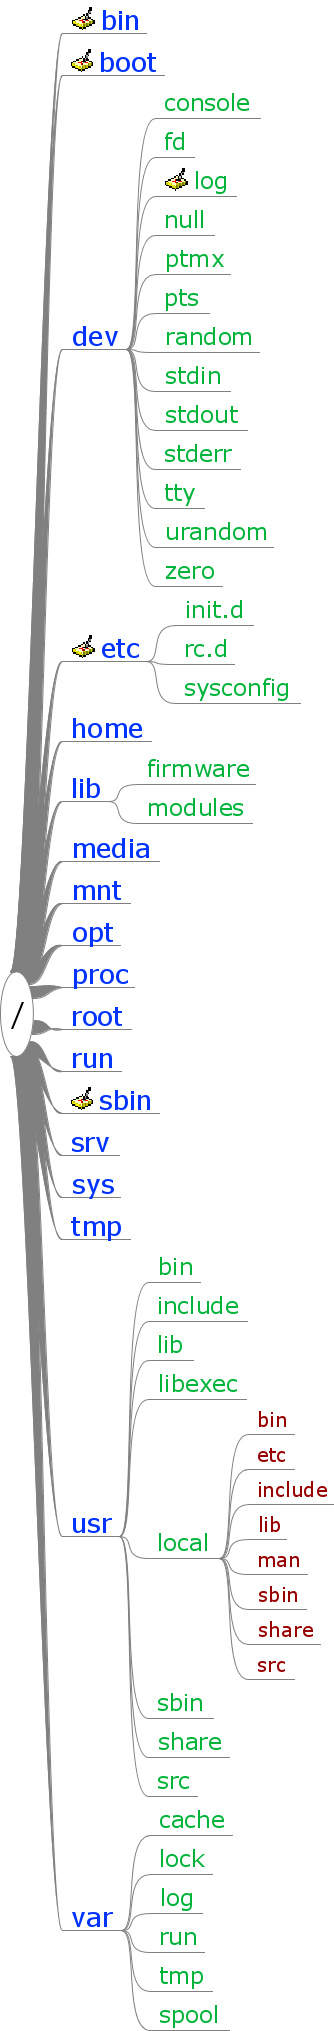
\includegraphics[height=0.8\textheight]{../../slides/fs/01-lhs.png}
	\column{0.7\textwidth}
		\begin{itemize}
			\item Директории
			\item Обычные файлы
			\item Симлинки
			\item Хардлинки
			\item Файлы устройств
			\item FIFO
			\item сокеты
		\end{itemize}
	\end{columns}
\end{frame}
}

\end{document}
